\section{System Design and Integration}\label{Sec:method}

% {\color{red}\textbf{Proposal:}}
% \begin{itemize}
%     \item In a concise way, present your solution and why you believe 
% this will improve upon the state-of-the-art. Include any 
% hardware and software proposal (either existing or new one) 
% that can be created/used for solving your problem.
% \end{itemize}

Through the background investigation, we found that good disinfection robots or medical robots should meet the characteristics of efficient work and flexible actions. We will also complete the system design according to the general needs and cognition of disinfection robots in the industry\cite{1717783}.

\subsection{Disinfection Robot Architecture Design}
\subsubsection{Mobile Base}
The base of a robot determines its flexibility, carrying capacity, and compact design. Because it needs to work in a complex and crowded environment, it is important to choose a suitable robot platform. According to the background investigation, we found that most medical robots are tall and thin, which helps them to work more like humans in sometimes crowded environments.\\
Thus, we choose Three-Mecanum-Wheel Configurations of the Mobile Robot (fig.\ref{tmw}). The base arranged in a circular array uses three wheels to better balance the load. The picture shows a common three mecanum wheel configuration. From the point of view of the intersection of the lower rollers, these configurations have omnidirectional movement performance. At the same time, the orthogonal Mecanum wheel is used for rotationally symmetrical configuration, which is usually used for indoor mobile service robots and light loading robots, which is very close to our needs.
\begin{figure}[htbp] 
\centering 
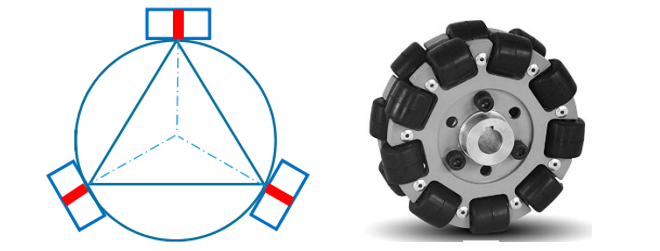
\includegraphics[width=0.45\textwidth]{figures/mwww.PNG} 
\caption{Three-Mecanum-Wheel-Base} 
\label{tmw} 
\end{figure}
\subsubsection{Robot Arm}
The reason for selecting this arm is that it can achieve full coverage and fine spraying, which effectively guarantees the coverage of disinfection, and the high DoF of the arm can ensure this. Thus, we choose to use Panda Robotic Arm\cite{gmbh_2021}, made by Franka Emika. There are several reasons for choosing it. First, it has a maximum load of 3.3kg, which satisfies the opportunity for us to perform secondary design on the end-effector of the arm. Secondly, its radius of activity is 855 mm, which satisfies the radius of most objects needed to disinfect in the hospital. At the same time, it can be perfectly compatible with ROS, and call SDKs such as movieit, which makes development convenient. Finally, after horizontal comparison, its cost performance is the highest, which also meets the requirements of large-scale production.\\
\par The overall structure is similar to RB-1 robotics (fig.\ref{rb-1}) created by Robotnik company\cite{rb-1robotnik2021}, but the Base should change to the one with Mecanum Wheels. Meanwhile, the alcohol container and hydraulic device required by spray gun will be installed on the back of the robot. There is also be a camera used for scanning modeling at the top, and the gyroscope and camera needed by SALM will be placed in front of the platform for identification. We will also install a circle of ultraviolet lights around the circular site, illuminating the ground at a designed angle, which is more conducive to the disinfection of the floor.
\begin{figure}[htbp] 
\centering 
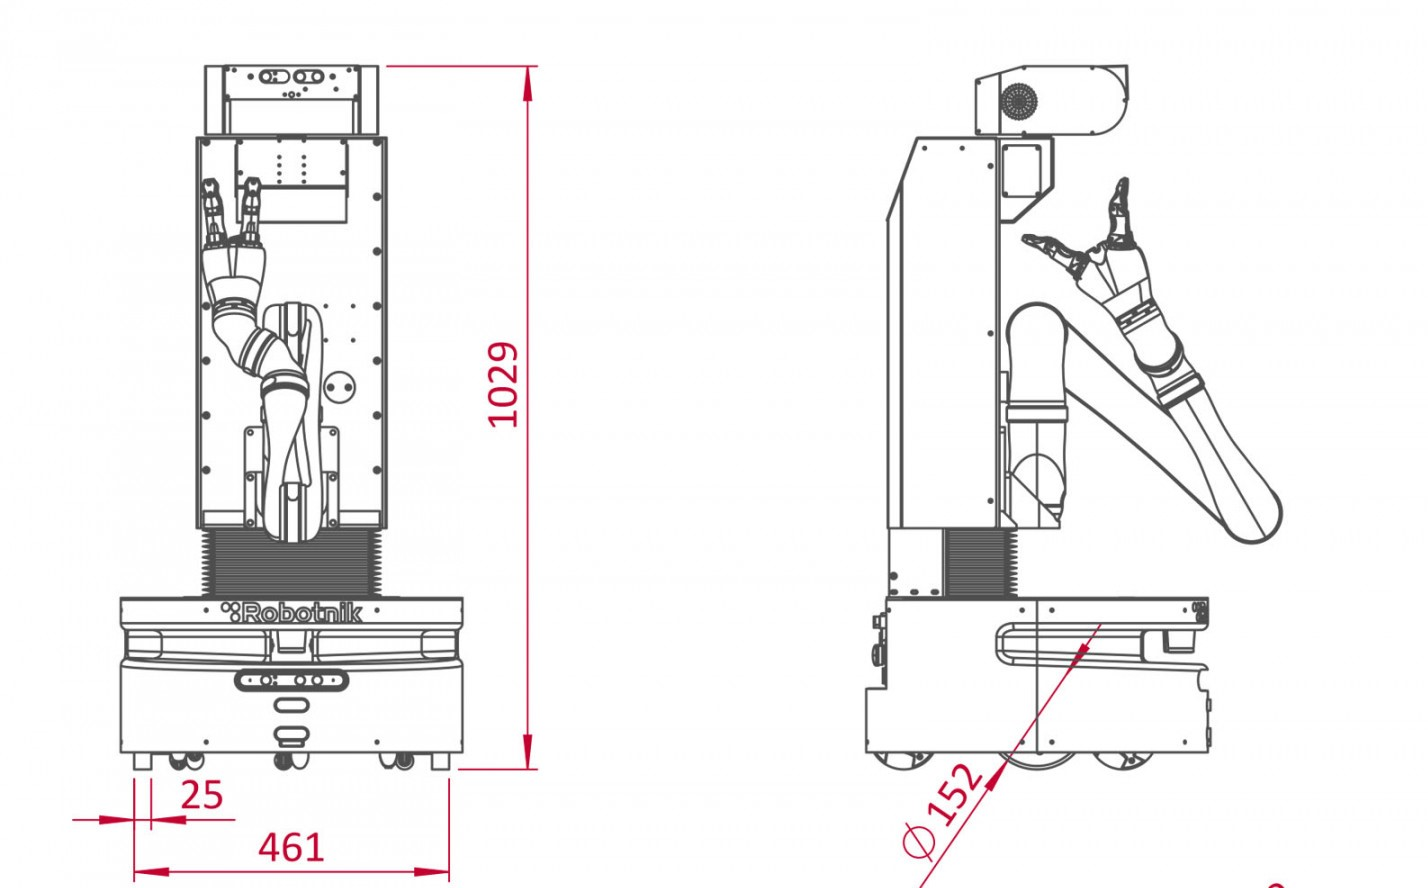
\includegraphics[width=0.45\textwidth]{figures/Robotnik-Cotas-RB-1-uai-1440x1387.jpg} 
\caption{RB-1 MOBILE MANIPULATOR} 
\label{rb-1} 
\end{figure}
\subsection{Movement Planning}
For a disinfection robot that automatically works in a hospital, mapping and localization are the basic requirements. Nowadays SLAM(Simultaneous Localization and Mapping) is an advanced and hottest technology to deal with this issue. Since SLAM was first proposed 30 years ago \cite{pritsker1984introduction}, it has gone through rapid development. In the future, the development of multi-sensors SLAM \cite{zhang2013application} and Semantic SLAM \cite{bowman2017probabilistic} can greatly improve the accuracy of mapping and localization which are good enough for the robot's work.
\par Also, the robot needs motion planning. It is divided into two parts, global planning and local planning. Global planning refers to a route that the robot moves on. Local planning refers to adjust itself when there are accidents during the movement. So far, to realize more complicated functions of service robot which is required to move in a more specific route and back to recharge when the battery is low, a topic named space coverage is researcher, one of the most famous algorithm and theory is called Morse Decompositions \cite{acar2002morse}. Based on this theory, the disinfection robot can divide the space then disinfect respectfully and recharge itself. 
              

\subsection{Multi-function End-effector Design}

In order to achieve full coverage spraying, we designed a switchable end-effector. In the background investigation, we found that the spraying shape is different according to the nozzle and pressure. According to the figure.\ref{spray pattern} \cite{ikeuchi_2021},
\begin{figure}[htbp] 
\centering 
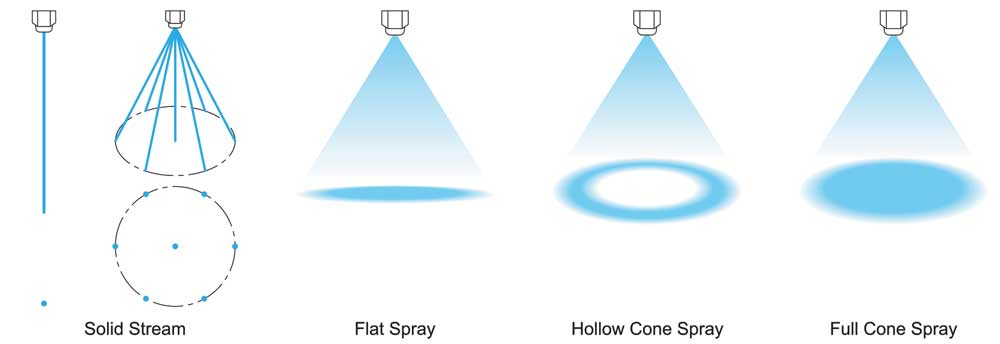
\includegraphics[width=0.5\textwidth]{figures/Spray-pattern.jpg} 
\caption{Spray Pattern} 
\label{spray pattern} 
\end{figure} 
we can see the most common spray patterns, according to different application scenarios, there will be different alcohol spraying solutions. For instance, when cleaning gaps or corners, we should use flat spray, and when spraying large areas, we should switch to a solid cone method. In order to integrate all the solutions, so as to achieve full coverage spraying, we have been inspired by the CNC machine tool and the lens converter of the microscope, and all the nozzles are assembled on a disc to form a cone, as shown in the figure.\ref{Nozzle Conversion Disc}, when the robot judges the different solutions are needed, just switch the nozzles to complete the corresponding tasks.


\begin{figure}[htbp] 
\centering 
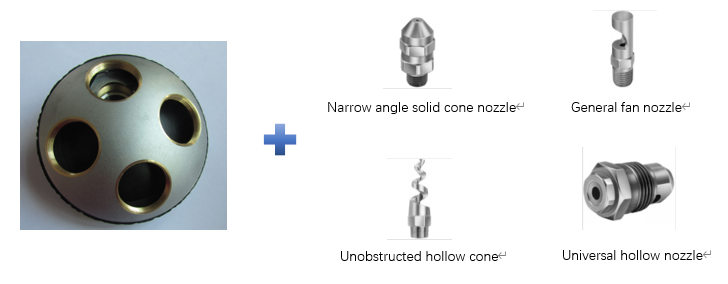
\includegraphics[width=0.5\textwidth]{figures/translator.PNG} 
\caption{Nozzle Conversion Disc} 
\label{Nozzle Conversion Disc} 
\end{figure}

\subsection{3D Scan Modeling and Control Method Design}
In the medical environment, disinfection of transparent glassware or plastic cups has always been very challenging. As a full-coverage disinfection robot, we have borrowed from the ClearGrasp algorithm(fig.\ref{3dshape})\cite{sajjan2020clear}, which is a deep learning method used to learn from a single RGB-D Estimate the accurate 3D geometry of transparent objects in the image for robot manipulation. Given an RGB-D image of a single transparent object, ClearGrasp uses a deep convolutional network to infer surface normals, masks and occlusion boundaries for transparent surfaces. These outputs are then used to optimize the initial depth estimate for all transparent surfaces in the scene. 
\par After obtaining the object model needed to spray and disinfect, we should plan the spraying path through graphic algorithms, which, analyzing the approximate shape of the object, and judge the edges and faces. Then manipulate the arms and the ground to reach these areas for work. Among algorithms for full-coverage scanning of known modeling. We recommend using DJI's PTZ fixed-point tracking algorithm\cite{dji}, which can identify the following objects in the air and follow the shooting 360 degrees. Applied it to our scene, it can spray around the known object from top to bottom so that cover all the exposed area of the object.
\begin{figure}[htbp] 
\centering 
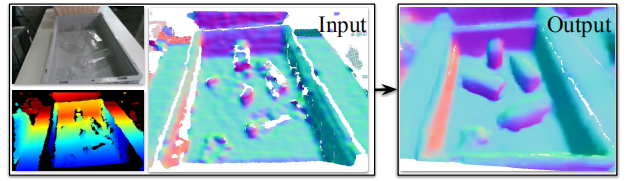
\includegraphics[width=0.45\textwidth]{figures/2020clear.png} 
\caption{3D Shape Estimation of Transparent Objects} 
\label{3dshape} 
\end{figure}